\section{Survival Distributions}
\label{sect:surv-dist}
\subsection{Future Lifetime Random Variable}
\begin{enumerate}
\item A life aged \(x\) (in years) is denoted by \((x)\).

\begin{note}
By ``aged \(x\)'', we mean the life's age is \emph{exactly} \(x\):

\begin{tikzpicture}
\draw[-Latex] (0,0) -- (10,0) node[right]{Age};
\fill[] (0,0) circle [radius=0.05]
node[above] {\faIcon{baby}}
node[below] {0};
\fill[] (2,0) circle [radius=0.05]
node[above] {\faIcon{birthday-cake}}
node[below] {1};
\fill[] (4,0) circle [radius=0.05]
node[above] {\faIcon{birthday-cake}}
node[below] {2};
\fill[] (6,0) circle [radius=0.05]
node[above] {\faIcon{birthday-cake}}
node[below] {3};
\fill[] (8,0) circle [radius=0.05]
node[above] {\faIcon{birthday-cake}}
node[below] {4};
\draw[-Latex] (1,1) node[above]{(0.5)} -- (1,0.2);
\draw[-Latex] (2.5,1) node[above]{(1.25)} -- (2.5,0.2);
\draw[-Latex] (5.5,1) node[above]{(2.75)} -- (5.5,0.2);
\draw[very thick, decorate,decoration={calligraphic brace, amplitude=5pt, raise=15pt, mirror}] (2.1,0) -- (3.8,0)
node[midway, below=0.7cm, font=\small]{``aged 1'' in daily life};
\end{tikzpicture}

From here we can see that ``age'' in daily life language actually refers to
number of birthdays passed, which is \emph{different} from our meaning.
\end{note}

\item \defn{Future lifetime random variable} for \((x)\) is a continuous
random variable \(T_x\) with support \([0,\infty)\).
\begin{note}
This means a life aged \(x\) cannot live forever, and the life ``almost never''
die exactly at age \(x\) (i.e., with probability 0).
\end{note}

\begin{tikzpicture}
\draw[-Latex] (0,0) -- (10,0) node[right]{Age};
\fill[] (0,0) circle [radius=0.05]
node[below] {0};
\fill[] (2,0) circle [radius=0.05]
node[below] {1};
\fill[] (4,0) circle [radius=0.05]
node[below] {2};
\fill[] (6,0) circle [radius=0.05]
node[below] {3};
\fill[] (8,0) circle [radius=0.05]
node[below] {4};
\fill[] (3.5,0) circle [radius=0.05]
node[below=0.05, font=\large] {\(x\)};
\node[] (life) at (3.5,0.3) {\faIcon{user}};
\draw[very thick, decorate,decoration={calligraphic brace, amplitude=5pt, raise=15pt}] (3.5,0) -- (9,0)
node[midway, above=0.7cm]{\(T_x\) (years)};
\node[red] (die) at (9, 0.3) {\faIcon{skull}};
\draw[-Latex] (8,-0.7) -- (die.south);
\node[] () at (8,-1) {age at death: \(x+T_x\)};
\end{tikzpicture}

\item The cdf of \(T_x\) (denoted by \(F_x(t)\)) is
\(F_x(t)=\prob{T_x\le t}\), which gives the probability that \((x)\) dies
within \(t\) years.

\item The survival function of \(T_x\) (denoted by \(S_x(t)\)) is
\(S_x(t)=\prob{T_x>t}\), which gives the probability that \((x)\) survives for
more than \(t\) years.

\item \label{it:key-assum} We would like to investigate the relationship between
distributions of \(T_0\) and \(T_x\) for the same ``underlying life'':

\begin{tikzpicture}
\draw[-Latex] (0,0) -- (10,0) node[right]{Age};
\fill[] (0,0) circle [radius=0.05]
node[above] (age0) {\faIcon{baby}}
node[below] {0};
\fill[] (2,0) circle [radius=0.05]
node[below] {1};
\fill[] (4,0) circle [radius=0.05]
node[below] {2};
\fill[] (6,0) circle [radius=0.05]
node[below] {3};
\fill[] (8,0) circle [radius=0.05]
node[below] {4};
\draw[very thick, decorate,decoration={calligraphic brace, amplitude=5pt, raise=15pt}] (0,0) -- (9,0)
node[midway, above=0.7cm]{\(T_0\)};
\end{tikzpicture}

\begin{tikzpicture}
\draw[-Latex] (0,0) -- (10,0) node[right]{Age};
\fill[] (0,0) circle [radius=0.05]
node[below] {0};
\fill[] (2,0) circle [radius=0.05]
node[below] {1};
\fill[] (4,0) circle [radius=0.05] node[below] {2};
\fill[] (6,0) circle [radius=0.05]
node[below] {3};
\fill[] (8,0) circle [radius=0.05]
node[below] {4};
\fill[] (3.5,0) circle [radius=0.05]
node[below=0.05, font=\large] {\(x\)};
\node[] (life) at (3.5,0.3) {\faIcon{user}};
\draw[very thick, decorate,decoration={calligraphic brace, amplitude=5pt, raise=15pt}] (3.5,0) -- (9,0)
node[midway, above=0.7cm]{\(T_x\)};
\end{tikzpicture}

\begin{note}
\faIcon{baby} and \faIcon{user} are the same life, but at different ages.
\end{note}

An ``internal'' information given implicitly is that \faIcon{baby}
survives to age \(x\) (since \((x)\) \emph{exists}!), i.e., the future lifetime
of \faIcon{baby} (\(T_0\)) is greater than \(x\).

Given this information, one may naturally expect \(T_0-x\) and \(T_x\) to have
the same distribution, as they appear to describe the same thing (how long
\faIcon{user} will live for). But a rather subtle difference between them is
the \emph{modelling time} of the distribution: the distribution of \(T_0-x\) is
to be modelled at age 0, while the distribution of \(T_x\) is to be modelled at
age \(x\).

With the absence of ``external'' information between age 0 and age \(x\), such
expectation is reasonable. However, if there is some relevant ``external''
information during the time interval (e.g., discovery of cancer cure), they
can have different distributions.

Nonetheless, to enrich the study of life contingencies, we shall impose the
assumption that for any age \(x\),
\[
(T_0-x|T_0>x)\eqd T_x.
\]

\begin{remark}
\item The assumption may be understood more intuitively as stating that, for any age
\(x\), (i) \(T_0\) and \(T_x\) have the same ``underlying life''; and (ii)
there is no ``external'' information between age 0 and age \(x\).
\item Expressing the assumption in terms of cdf, we have:
\[
\prob{T_x\le t}=\prob{T_0\le x+t|T_0>x}.
\]
\end{remark}
\item Having the assumption in \labelcref{it:key-assum}, we can derive the
following results:
\begin{proposition}
\label{prp:chain-surv}
\(S_0(x+t)=S_0(x)S_x(t)\) for any age \(x\) and \(t\ge 0\).
\end{proposition}

\begin{intuition}
LHS means ``(0) lives for \(x+t\) years'', and RHS means ``(0) lives for \(x\)
years (becoming (\(x\))), and then lives for \(t\) more years'', so LHS and RHS
``should'' be the same.\footnote{Generally, this kind of ``intuition'' is very helpful in the study of
life contingencies.}

\begin{tikzpicture}
\draw[-Latex] (0,0) -- (10,0) node[right]{Age};
\fill[] (0,0) circle [radius=0.05]
node[below] {0};
\fill[] (3,0) circle [radius=0.05]
node[below=0.05, font=\large] {\(x\)};
\fill[] (7,0) circle [radius=0.05]
node[below=0.05, font=\large] {\(x+t\)};
\draw[-Latex] (0,0.2) to[bend left] (3,0.2);
\draw[-Latex] (3,0.2) to[bend left] (7,0.2);
\node[] () at (1.5, 1) {lives for \(x\) years};
\node[] () at (5, 1) {lives for \(t\) more years};
\draw[-Latex] (0,-0.5) to[bend right] (7,-0.5);
\node[] () at (3.5, -1) {lives for \(x+t\) years};
\end{tikzpicture}
\end{intuition}

\begin{note}
This ``and-then'' intuition is ``justified'' because of the assumption in
\labelcref{it:key-assum}.
\end{note}

\begin{pf}
Note that
\[
\prob{T_0\le x+t|T_0>x}=\frac{\prob{x<T_0\le x+t}}{\prob{T_0>x}}
=\frac{S_0(x)-S_0(x+t)}{S_0(x)}
=1-\frac{S_0(x+t)}{S_0(x)},
\]
and
\[
\prob{T_x\le t}=1-S_x(t).
\]
So, we have
\[
\prob{T_x\le t}=\prob{T_0\le x+t|T_0>x}
\implies 
S_x(t)=\frac{S_0(x+t)}{S_0(x)},
\]
as desired.
\end{pf}

\begin{proposition}
\label{prp:gen-chain-surv}
\(S_x(t+u)=S_x(t)S_{x+t}(u)\) for any age \(x\) and any \(t,u\ge 0\).
\end{proposition}

\begin{intuition}
LHS means ``(\(x\)) lives for \(t+u\) years'', and RHS means ``(\(x\)) lives
for \(t\) years, and then lives for \(u\) more years'', so LHS and RHS
``should'' be the same.

\begin{tikzpicture}
\draw[-Latex] (0,0) -- (10,0) node[right]{Age};
\fill[] (0,0) circle [radius=0.05]
node[below] {0};
\fill[] (1,0) circle [radius=0.05]
node[below=0.05, font=\large] {\(x\)};
\fill[] (4,0) circle [radius=0.05]
node[below=0.05, font=\large] {\(x+t\)};
\fill[] (8,0) circle [radius=0.05]
node[below=0.05, font=\large] {\(x+t+u\)};
\draw[-Latex] (1,0.2) to[bend left] (4,0.2);
\draw[-Latex] (4,0.2) to[bend left] (8,0.2);
\node[] () at (2.5, 1) {lives for \(t\) years};
\node[] () at (6, 1) {lives for \(u\) more years};
\draw[-Latex] (1,-0.5) to[bend right] (8,-0.5);
\node[] () at (4.5, -1) {lives for \(t+u\) years};
\end{tikzpicture}
\end{intuition}

\begin{pf}
Applying the result in \cref{prp:chain-surv} to LHS and RHS gives
respectively
\[
\frac{S_0(x+t+u)}{S_0(x)}\text{ and }
\frac{S_0(x+t)}{S_0(x)}\cdot\frac{S_0(x+t+u)}{S_0(x+t)}
\]
which are clearly identical.
\end{pf}

\begin{note}
From here we can deduce that
\[
\prob{T_x>t+u}=\prob{T_x>t}\prob{T_{x+t}>u}
\implies
\prob{T_x>t+u|T_x>t}=\prob{T_{x+t}>u},
\]
which implies \((T_x-t|T_x>t)\eqd T_{x+t}\), a ``generalization'' to our
assumption in \labelcref{it:key-assum}.
\end{note}

\item \label{it:valid-surv} To model the distribution of future lifetime, we often specify a
\emph{survival function} (which can completely determine a probability
distribution). Thus, we are interested in studying what conditions on a
function are needed for it to qualify as a survival function for the future
lifetime, so that we know whether our choice of ``survival function'' is
reasonable or not.

\begin{proposition}
\label{prp:valid-surv}
A function \(S_x\) defined on \([0,\infty)\) is a valid survival function
for the future lifetime iff the following hold:
\begin{enumerate}
\item[(S1)] \(S_x(0)=1\);
\item[(S2)] \(\lim_{t\to \infty}S_x(t)=0\);
\item[(S3)] \(S_x(t)\) is a nondecreasing function of \(t\).
\end{enumerate}
\end{proposition}

\begin{intuition}
(S1) reflects that a life aged \(x\) cannot be dead at age \(x\). (S2) means
that all lives eventually die. (S3) respects the monotonicity property of
probability.
\end{intuition}

\item \label{it:additional-cond}
For mathematical convenience, we shall impose the following additional
conditions on \(S_x\):
\begin{enumerate}
\item \(S_x(t)\) is differentiable at any \(t>0\) (except possibly at some
``edge'' points)
\item \(\lim_{t\to \infty}tS_x(t)=0\).
\item \(\lim_{t\to \infty}t^2S_x(t)=0\).
\end{enumerate}
\begin{remark}
\item The latter two conditions are mainly useful for ensuring the existence of mean
and variance of \(T_x\).
\item For survival functions introduced here, they all satisfy these conditions
as well as the properties in \labelcref{it:valid-surv}.
\end{remark}
\end{enumerate}
\subsection{Force of Mortality}
\begin{enumerate}
\item Recall that the \emph{force of interest} at time \(t\) (\(\delta_t\)) can
be seen as ``relative'' rate of change of amount function \(A(\cdot)\):
\[
dA(t)=A(t)\delta_tdt,\quad\text{or}\quad
\delta_t=\frac{A'(t)}{A(t)},
\]
where \(A(t)\delta_tdt\) may be understood intuitively as ``interest earned in
\([t,t+dt]\)''.

\item Since force of mortality is also a ``force'', one may expect it is also
defined as relative rate of change of some function. A natural choice may be
the survival function \(S_0\) (for force of mortality ``modelled'' at age 0).
But as ``mortality'' is opposite to ``survival'', it appears that we should add
a negative sign in the definition.

\item \label{it:fom} The \defn{force of mortality (``modelled'' at age 0)} at
time \(t\), denoted by \(\mu_t\) (or \(\mu_0(t)\)), is defined as
\[
\mu_t=-\frac{S_0'(t)}{S_0(t)}.
\]
\begin{intuition}
We can express this as \(dS_0(t)=-S_0(t)\mu_tdt\), and \(S_0(t)\mu_tdt\) may be
intuitively understood as ``drop in survival probability in \([t,t+dt]\)'' or
``probability of death in \([t,t+dt]\)''.

\begin{tikzpicture}
\draw[-Latex] (0,0) -- (10,0) node[right]{Age};
\fill[] (0,0) circle [radius=0.05]
node[below] {0};
\fill[] (3,0) circle [radius=0.05]
node[below left] {\(t\)};
\fill[] (3.1,0) circle [radius=0.05]
node[below right] {\(t+dt\)};
\draw[-Latex] (0,0.2) to[bend left] (3,0.2);
\node[] () at (1.5, 1) {lives for \(t\) years};
\draw[color=red,decorate,decoration={brace, amplitude=5pt}] (3, 0.2) -- (3.1,0.2)
node[midway, above=0.3cm]{\faIcon{skull}};
\end{tikzpicture}
 \end{intuition}
\item Denote by \(f_x(t)\) the pdf of \(T_x\). Then, we have:
\begin{proposition}
\label{prp:mu-pdf-0}
\[
\mu_t=\frac{f_0(t)}{S_0(t)}
\]
for any \(t>0\).
\end{proposition}

\begin{note}
This explains why the intuition in \labelcref{it:fom} works: because
\(S_0(t)\mu_tdt=f_0(t)dt\).
\end{note}

\begin{pf}
The result follows from noting that
\[
-\frac{d}{dt}S_0(t)
=-\frac{d}{dt}(1-F_0(t))
=-(-f_0(t))
=f_0(t).
\]
\end{pf}

\item Now we would like to extend the concept of force of mortality to the case
where it can be ``modelled'' at any age \(x\). The definition is analogous: The
\defn{force of mortality (``modelled'' at age \(x\))} at time \(t\), denoted by
\(\mu_x(t)\), is
\[
\mu_x(t)=-\frac{S_x'(t)}{S_x(t)}.
\]

\begin{tikzpicture}
\draw[-Latex] (0,0) -- (10,0) node[right]{Age};
\fill[] (0,0) circle [radius=0.05]
node[below] {0};
\fill[] (3,0) circle [radius=0.05]
node[below=0.05cm] {\(x\)};
\fill[] (7,0) circle [radius=0.05]
node[below left] {\(x+t\)};
\fill[] (7.1,0) circle [radius=0.05]
node[below right] {\(x+t+dt\)};
\draw[-Latex] (3,0.2) to[bend left] (7,0.2);
\node[] () at (5, 1) {lives for \(t\) years};
\draw[color=red,decorate,decoration={brace, amplitude=5pt}] (7, 0.2) -- (7.1,0.2)
node[midway, above=0.3cm]{\faIcon{skull}};
\end{tikzpicture}

A natural question arised is whether \(\mu_x(t)=\mu_{x+t}\) or not.
\begin{note}
The latter one is to be regarded as the force of mortality at time \(x+t\)
(``modelled'' at age 0) here:

\begin{tikzpicture}
\draw[-Latex] (0,0) -- (10,0) node[right]{Age};
\fill[] (0,0) circle [radius=0.05]
node[below] {0};
\fill[] (3,0) circle [radius=0.05]
node[below=0.05cm] {\(x\)};
\fill[] (7,0) circle [radius=0.05]
node[below left] {\(x+t\)};
\fill[] (7.1,0) circle [radius=0.05]
node[below right] {\(x+t+dt\)};
\draw[-Latex] (0,0.2) to[bend left] (7,0.2);
\node[] () at (3.5, 1.5) {lives for \(x+t\) years};
\draw[color=red,decorate,decoration={brace, amplitude=5pt}] (7, 0.2) -- (7.1,0.2)
node[midway, above=0.3cm]{\faIcon{skull}};
\end{tikzpicture}
\end{note}

Fortunately, this is the case:

\begin{pf}
Firstly,
\[
\frac{d}{dt}S_x(t)
=\frac{d}{dt}\frac{S_0(x+t)}{S_0(x)}
=\frac{1}{S_0(x)}\frac{d}{dt}S_0(\underbrace{x+t}_{u})
=\frac{S_0'(u)}{S_0(x)}\underbrace{\frac{du}{dt}}_{1},
\]
and
\[S_x(t)=\frac{S_0(u)}{S_0(x)}.\]
So,
\[
\mu_x(t)=-\frac{S_0'(u)/S_0(x)}{S_0(u)/S_0(x)}
=-\frac{S_0'(u)}{S_0(u)}=\mu_u=\mu_{x+t}.
\]
\end{pf}

In view of this, we can simply use the notation ``\(\mu_{x+t}\)'' to stand for
either meaning without ambiguity.

\item One would then expect the following result holds also:
\begin{proposition}
\label{prp:mu-pdf-x}
\[
\mu_{x+t}=\frac{f_x(t)}{S_x(t)}
\]
for any age \(x\) and \(t>0\).
\end{proposition}
\begin{pf}
Replace ``0'' in the proof of \cref{prp:mu-pdf-0} by \(x\).
\end{pf}

\item Recall that for force of interest, we have
\[
A(t)=A(0)\exp\qty(\int_{0}^{t}\delta_s\,ds).
\]
As force of mortality is defined similarly, we may anticipate similar results
hold for force of mortality, and this is the case:
\begin{note}
Recall that \(S_x(0)=1\).
\end{note}
\begin{proposition}
\label{prp:sx-int}
\[
S_x(t)=\exp\qty(-\int_{0}^{t}\mu_{x+s}\,ds)
\]
for any age \(x\) and \(t>0\).
\end{proposition}

\begin{intuition}
Firstly, since force of mortality is defined similarly as force of interest, we
have analogously \(S_x(t)=e^{{\color{red}-}\mu t}\) if the force of mortality is
\emph{constant} (\(\mu_x(t)=\mu_{x+t}=\mu\) for any \(t>0\)). Then, when
\(h>0\) is small, we would have
\[
S_x(s+h)\approx S_x(s)e^{-\mu_{x+s} h}
\]
(during a ``small'' time interval \([s, s+h]\), the force of mortality is
``approximately'' constant). Thus,
\[
S_x(t)=\frac{S_x(h)}{S_x(0)}\frac{S_x(2h)}{S_x(h)}\frac{S_x(3h)}{S_x(2h)}\cdots\frac{S_x(t)}{S_x(t-h)}
\approx \exp\qty[-(\mu_{x}h+\mu_{x+h} h+\mu_{x+2h} h+\dotsb+\mu_{x+t-h}h)],
\]
and loosely, as \(h\to 0^+\), we have
\[
S_x(t)=\exp\qty(-\int_{0}^{t}\mu_{x+s}\,ds).
\]
\end{intuition}

\begin{pf}
Note that \(\displaystyle\mu_{x}(s)=\frac{d}{ds}\ln S_x(s)\). Then, taking
integral on both sides and applying fundamental theorem of calculus give the
desired result.
\end{pf}

\item \label{it:fom-spec-dist} By \cref{prp:sx-int}, if we know \(\mu_y\) for
any \(y\in[x, x+t]\), \(S_x(t)\) is determined. Hence, once \(\mu_y\) is known
for any \(y\ge x\) (so \(S_x(t)\) is determined for any \(t\ge 0\)), the
distribution of \(T_x\) is \emph{completely specified}.

\item In view of \labelcref{it:fom-spec-dist}, an alternative way to model the
distribution of future lifetime is to specify the force of mortality at
different time. There are some typical specifications of force of mortality
(which completely determine the future lifetime's distribution), called
\defn{mortality laws} (they govern the ``behaviour'' of mortality).

\item Here we discuss some mortality laws:
\begin{enumerate}
\item Gompertz
\item Makeham
\item (Generalized) De Movire
\item Constant Force of Mortality
\end{enumerate}

\item \defn{Gompertz's Law} is defined by
\[
\mu_x=Bc^x,\quad \text{where }B>0, c>1.
\]

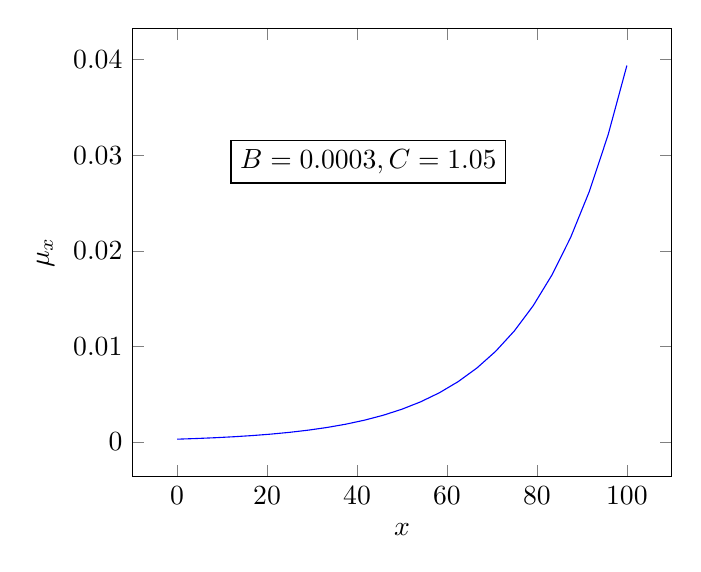
\begin{tikzpicture}
	\begin{axis}[domain=0:100, xlabel=\(x\), ylabel=\(\mu_x\), scaled y ticks=false, /pgf/number format/fixed]
		\addplot[blue] {0.0003*1.05^x};
	\end{axis}
\node[draw] () at (3,4) {\(B=0.0003, C=1.05\)};
\end{tikzpicture}

\item \defn{Makeham's Law} (genealization to Gompertz's law) is defined by
\[
\mu_x=A+Bc^x,\quad \text{where }A,B>0, c>1.
\]

\begin{tikzpicture}
	\begin{axis}[domain=0:100, xlabel=\(x\), ylabel=\(\mu_x\), scaled y ticks=false, /pgf/number format/fixed, ymin=0]
		\addplot[blue] {0.005+0.0003*1.05^x};
	\end{axis}
\node[draw] () at (3,5) {\(A=0.005, B=0.0003, C=1.05\)};
\draw[fill] (0.6,0.6) circle [radius=0.05];
\draw[color=red, thick, decorate,decoration={mirror, brace, amplitude=5pt}] (0.6, 0.5) -- (0.6,0);
\draw[color=red, thick, decorate,decoration={mirror, brace, amplitude=5pt}] (4.6, 0.5) -- (4.6,0);
\draw[color=red, thick, decorate,decoration={mirror, brace, amplitude=5pt}] (5.6, 0.5) -- (5.6,0);
\draw[fill] (4.6,1.7) circle [radius=0.05];
\draw[fill] (5.6,3.15) circle [radius=0.05];
\draw[color=brown, thick, decorate,decoration={brace, amplitude=5pt}] (4.6, 0.5) -- (4.6,1.7);
\draw[color=brown, thick, decorate,decoration={brace, amplitude=5pt}] (5.6, 0.5) -- (5.6,3.15);
\draw[-Latex] (8,-1) -- (0.6, 0.3);
\draw[-Latex] (8,-1) -- (4.6, 0.3);
\draw[-Latex] (8,-1) -- (5.6, 0.3);
\node[] () at (8.5,-1.3) {``accidental'' force of mortality};
\draw[-Latex] (8,3) -- (4.6, 1.3);
\draw[-Latex] (8,3) -- (5.6, 2);
\node[] () at (9,3.3) {``natural'' force of mortality};
\end{tikzpicture}

The constant \(A\) reflects the risk of \emph{accidental death}, which is
supposed to be constant for any age.

\item \defn{De Moivre's Law} is defined by
\[
\mu_x=\frac{1}{\omega-x}, \quad\text{where }0\le x<\omega
\]
and the \defn{generalized De Moivre's Law} is defined by
\[
\mu_x=\frac{\alpha}{\omega-x}, \quad\text{where }0\le x<\omega, \alpha>0.
\]

\begin{tikzpicture}
	\begin{axis}[domain=0:99, xlabel=\(x\), ylabel=\(\mu_x\), scaled y ticks=false, /pgf/number format/fixed, samples=100]
	\addplot[blue] {1/(100-x)};
	\end{axis}
\node[draw] () at (3,3) {\(\alpha=1,\omega=100\)};
\draw[-Latex, red] (8,1) -- (6.5,2);
\node[text width=3cm] () at (9,0.3) {``sudden'' surge in force of mortality near \(\omega\)};
\end{tikzpicture}

\item \label{it:de-moivre-dist-surv}
For De Moivre's law, the survival function is given by
\[
S_x(t)=\exp\qty(\int_{0}^{t}\mu_{x+s}\,ds)
=1-\frac{t}{\omega-x},\quad\text{where }0 \le t<\omega-x.
\]
Note that \(\lim_{t\to \omega-x}S_x(t)=0\), which suggests that as the age of a
life appraoches \(\omega\), his surviving probability approaches 0, so
\(\omega\) can be seen as a ``limiting age''.

To ensure the survival function to be valid (i.e., satisfies the properties
mentioned in \labelcref{it:valid-surv}), we can only set \(S_x(t)=0\) for any
\(t\ge \omega-x\). This implies that under De Moivre's Law, the future lifetime
random variable \(T_x\sim U[0,\omega-x]\).

\begin{note}
The survival function \(S_x(t)\) is not differentiable at the
``edge'' point \(t=\omega-x\).

\begin{tikzpicture}
[
declare function={
func(\x) = (\x < 50) * (1-x/50) + (\x >= 50) * 0;
}
]
\begin{axis}[domain=0:75, xlabel=\(t\), ylabel=\(S_{50}(t)\)]
\addplot[blue]{func(x)};
\end{axis}
\node[draw] () at (5,3) {\(\alpha=1,\omega=100\)};
\node[] () at (8.5,3) {not differentiable};
\draw[-Latex] (8,2.5) -- (4.5,0.7);
\draw[fill, red] (4.4,0.48) circle [radius=0.05];
\end{tikzpicture}
\end{note}

\item \label{it:gen-de-moivre-surv}
For generalized De Moivre's Law, the survival function is
\[
S_x(t)=\exp\qty(\alpha\int_{0}^{t}\frac{1}{\omega-x-s}\,ds)
=\qty(1-\frac{t}{\omega-x})^{\alpha},\quad\text{where }0 \le t<\omega-x.
\]
Likewise, we can only have \(S_x(t)=0\) for any \(t\ge\omega-x\).
\item Lastly, for \defn{constant force of mortality}, as its name suggests, it assumes
\[
\mu_x=\mu
\]
for any age \(x\), where \(\mu>0\) is a constant.
In this case, by \cref{prp:sx-int}, the survival function is given by
\[
S_x(t)=e^{-\mu t}
\]
for any \(t\ge 0\), so the future lifetime random variable
\(T_x\sim\mathrm{Exp}(\mu)\) (for any age \(x\)).
\end{enumerate}
\subsection{Actuarial Notations}
\begin{enumerate}
\item Here we introduce actuarial notations for concepts discussed before.
\item Two main kinds of actuarial notations here: ``\(p\)'' (probability
related to ``survival'') and ``\(q\)'' (probability related to ``death'').
\item \label{it:actuar-pq} A list of actuarial notations:
\begin{itemize}
\item \(\px[t]{x}\): \(S_x(t)\)
\item \(\qx[t]{x}\): \(F_x(t)\)
\item \(\qx[u|t]{x}\): \(\prob{u<T_x\le u+t}=S_x(u)-S_x(u+t)\)
\end{itemize}
\begin{remark}
\item ``\(t\)'' can be dropped from the notation if \(t=1\), for simplicity.
\item For ``\(u|t\)'', \(u\) is the length of deferment period, and \(t\) is
the length of period following the deferment.
\begin{tikzpicture}
\draw[-Latex] (0,0) -- (10,0) node[right]{Time};
\fill[] (0,0) circle [radius=0.05]
node[below] {0}
node[above] {\((x)\)};
\fill[] (3,0) circle [radius=0.05]
node[below] {\(u\)};
\fill[] (5,0) circle [radius=0.05]
node[below] {\(u+t\)};
\draw[very thick, decorate,decoration={calligraphic brace, amplitude=5pt, raise=10pt}] (3,0) -- (5,0)
node[midway, above=0.7cm]{die (\(\qx[u|t]{x}\))};
\draw[very thick, decorate,decoration={calligraphic brace, mirror,  amplitude=5pt, raise=12pt}] (0,0) -- (3,0)
node[midway, below=0.7cm]{deferment period};
\end{tikzpicture}
\end{remark}

\item Based on the definitions in \labelcref{it:actuar-pq}, we can readily
derive the following formulas:
\begin{proposition}
\label{prp:act-notation-prop}
For any age \(x\) and \(t,u\ge 0, n\in\N\),
\begin{enumerate}
\item \(\px[t]{x}+\qx[t]{x}=1\).
\begin{intuition}
(\(x\)) either dies within or survive for \(t\) years.
\end{intuition}
\item \(\px[t+u]{x}=\px[t]{x}\,\px[u]{x+t}\),
\begin{note}
This is just \cref{prp:gen-chain-surv} expressed in actuarial notations.\
\end{note}\\
and
\(\px[n]{x}=\px{x}\px{x+1}\cdots\px{x+n-1}\).
\begin{note}
This can be obtained by applying the former result repetitively.
\end{note}
\item \(\qx[u|t]{x}=\px[u]{x}-\px[u+t]{x}\).
\begin{intuition}

\begin{tikzpicture}
\node[] () at (-2,0) {(LHS)};
\draw[-Latex] (0,0) -- (10,0) node[right]{Time};
\fill[] (0,0) circle [radius=0.05]
node[below] {0}
node[above] {\((x)\)};
\fill[] (3,0) circle [radius=0.05]
node[below] {\(u\)};
\fill[] (5,0) circle [radius=0.05]
node[below] {\(u+t\)};
\draw[very thick, decorate,decoration={calligraphic brace, amplitude=5pt, raise=10pt}] (3,0) -- (5,0)
node[midway, above=0.7cm]{die};
\end{tikzpicture}

\begin{tikzpicture}
\node[] () at (-2,0) {(RHS)};
\draw[-Latex] (0,0) -- (10,0) node[right]{Time};
\fill[] (0,0) circle [radius=0.05]
node[below] {0}
node[above] {\((x)\)};
\fill[] (3,0) circle [radius=0.05]
node[below] {\(u\)};
\fill[] (5,0) circle [radius=0.05]
node[below] {\(u+t\)};
\draw[very thick, decorate,decoration={mirror, calligraphic brace, amplitude=5pt, raise=10pt}] (3,0) -- (10,0)
node[midway, below=0.7cm]{die somewhere};
\draw[very thick, decorate,decoration={calligraphic brace, amplitude=5pt, raise=10pt}] (5,0) -- (10,0)
node[midway, above=0.7cm]{but not die here};
\end{tikzpicture}

\end{intuition}
\item \(\qx[u|t]{x}=\qx[u+t]{x}-\qx[u]{x}\).
\begin{intuition}

\begin{tikzpicture}
\node[] () at (-2,0) {(LHS)};
\draw[-Latex] (0,0) -- (10,0) node[right]{Time};
\fill[] (0,0) circle [radius=0.05]
node[below] {0}
node[above] {\((x)\)};
\fill[] (3,0) circle [radius=0.05]
node[below] {\(u\)};
\fill[] (5,0) circle [radius=0.05]
node[below] {\(u+t\)};
\draw[very thick, decorate,decoration={calligraphic brace, amplitude=5pt, raise=10pt}] (3,0) -- (5,0)
node[midway, above=0.7cm]{die};
\end{tikzpicture}

\begin{tikzpicture}
\node[] () at (-2,0) {(RHS)};
\draw[-Latex] (0,0) -- (10,0) node[right]{Time};
\fill[] (0,0) circle [radius=0.05]
node[below] {0}
node[above] {\((x)\)};
\fill[] (3,0) circle [radius=0.05]
node[below] {\(u\)};
\fill[] (5,0) circle [radius=0.05]
node[below] {\(u+t\)};
\draw[very thick, decorate,decoration={mirror, calligraphic brace, amplitude=5pt, raise=12pt}] (0,0) -- (5,0)
node[midway, below=0.7cm]{die somewhere};
\draw[very thick, decorate,decoration={calligraphic brace, amplitude=5pt, raise=15pt}] (0,0) -- (3,0)
node[midway, above=0.7cm]{but not die here};
\end{tikzpicture}

\end{intuition}
\item \(\qx[u|t]{x}=\px[u]{x}\,\qx[t]{x+u}\).
\begin{intuition}
Dies in time interval \([u, u+t]\) = First survives for \(u\) years, \emph{and then}
dies within the coming \(t\) years.
\end{intuition}
\item \(f_x(t)=\px[t]{x}\mu_{x+t}\).
\begin{intuition}
Similar to the intuition in \labelcref{it:fom}, \(\px[t]{x}\mu_{x+t}dt\) may be
interpreted ``probability of death in time interval \([t,t+dt]\)''. On the
other hand, \(f_x(t)dt\) may also be understood as ``probability of death in
time interval \([t,t+dt]\)''.
\end{intuition}
\end{enumerate}
\end{proposition}

\item Intuitively, ``\(q\)'' and ``\(\mu\)'' are respectively describing death
``discretely'' and ``continuously'' (analogous to ``\(i\)'' and ``\(\delta\)''
in STAT2902).

\item The relationship between ``\(q\)'' and ``\(\mu\)'' is given by:
\begin{proposition}
\label{prp:qx-int}
\[
\qx[t]{x}=\int_{0}^{t}\px[s]{x}\mu_{x+s}\,ds
\]
for any age \(x\) and \(t\ge 0\).

\begin{intuition}
RHS ``sums up'' the ``probabilities of death'' in all ``infinitesimal'' time
intervals within the interval \([0,t]\).
\end{intuition}
\end{proposition}
\end{enumerate}

\subsection{Mean and Variance of \(T_x\)}
\begin{enumerate}
\item The \defn{complete expectation of life} is \(\expv{T_x}\). (Actuarial
notation: \(\eringx{x}\))

\begin{remark}
\item ``Complete'' is in the sense that the ``complete'' (``whole'') lifetime is
considered in the calculation (and not, say, just the integer part of
lifetime).
\item By the conditions in \labelcref{it:additional-cond}, \(\eringx{x}\) exists.
\end{remark}

\item By definition, we have
\[
\eringx{x}=\int_{0}^{\infty}t\,\px[t]{x}\mu_{x+t}\,dt.
\]
However, this is a bit complicated to evaluate and we almost always use the
following simpler formula instead:
\begin{proposition}
\label{prp:eringx-fmla}
\[
\eringx{x}=\int_0^{\infty}\px[t]{x}\,dt.
\]
\end{proposition}

\begin{pf}
Since \(T_x\) is nonnegative, we have
\[
T_x=\int_{0}^{T_x}1\,dt
=\int_{0}^{\infty}\indicset{t<T_x}\,dt.
\]
\begin{note}
\(\indicset{\cdot}\) denotes the indicator function.
\end{note}

It then follows that
\[
\expv{T_x}=\expv{\int_{0}^{\infty}\indicset{t<T_x}\,dt}
=\int_{0}^{\infty}\expv{\indicset{T_x>t}}\,dt
=\int_{0}^{\infty}\prob{T_x>t}\,dt,
\]
as desired. (The second equality holds by Fubini's theorem.)
\end{pf}

\item To find the \emph{variance} of \(T_x\), we need to compute the second
moment of \(T_x\): \(\expv{T_x^2}\) (again its existence is guaranteed by the
conditions in \labelcref{it:additional-cond}).
\item Likewise we almost always use the following alternative formula instead
of the definition:
\begin{proposition}
\label{prp:tx-2nd-moment-fmla}
\[
\expv{T_x^2}=2\int_{0}^{\infty}t\,\px[t]{x}\,dt.
\]
\end{proposition}
\begin{pf}
By definition, we have:
\[
\expv{T_x^2}=\int_{0}^{\infty}t^2\px[t]{x}\mu_{x+t}\,dt
=-\int_{0}^{\infty}t^2\frac{d}{dt}\px[t]{x}\,dt.
\]
Integrating it by parts gives
\[
\underbrace{-[t^2\px[t]{x}]_0^{\infty}}_{0}-\int_{0}^{\infty}2t\px[t]{x}\,dt
\]
where the first term is zero due to the conditions in
\labelcref{it:additional-cond}.
\end{pf}

Once we compute the first and second moments of \(T_x\): \(\expv{T_x}\) and
\(\expv{T_x^2}\), we can find the variance of \(T_x\) by
\[
\vari{T_x}=\expv{T_x^2}-\qty(\expv{T_x})^2.
\]

\item Sometimes we are interested in the future lifetime random variable
``capped'' to \(n\) years: \(T_x\wedge n\) (i.e.,
\(\min\{T_x, n\}\)) (e.g., in the context of endowment insurance; see later
sections). The expectation of this capped random variable (i.e.,
\(\expv{T_x\wedge n}\)) is called the \defn{term expectation of life}.
(Actuarial notation: \(\eringx{\endowxn}\))

\begin{note}
The notation ``\(\endowxn\)'' is used when the ``capped'' future lifetime
random variable \(T_x\wedge n\) is involved. Abusing the notation a bit, we may
actually write \(T_x\wedge n\) as ``\(T_{\endowxn}\)'', and regard the latter
as ``another future lifetime random variable'' where ``standard'' actuarial
notations apply (this will be useful in some later sections here, and more
details will be explained in STAT3909).
\end{note}

\item Similarly we have the following formula for \(\eringx{\endowxn}\):
\begin{proposition}
\label{prp:eringxn-fmla}
\[
\eringx{\endowxn}=\int_{0}^{n}\px[t]{x}\,dt.
\]
\end{proposition}
\begin{pf}
Replace \(T_x\) by \(T_x\wedge n\) in the proof of \cref{prp:eringx-fmla}, and note that
\[
\expv{\int_{0}^{\infty}\indicset{t<T_x\wedge n}\,dt}
=\expv{\int_{0}^{\infty}\indicset{t<T_x}\indicset{t<n}\,dt}
=\expv{\int_{0}^{n}\indicset{t<T_x}\,dt}.
\]
\end{pf}
\end{enumerate}
\subsection{Curtate Future Lifetime Random Variable}
\begin{enumerate}
\item Recall the discrepancy between the meaning of ``age'' here (exact) versus
the daily life meaning (number of birthdays passed):

\begin{tikzpicture}
\draw[-Latex] (0,0) -- (10,0) node[right]{Age};
\fill[] (0,0) circle [radius=0.05]
node[above] {\faIcon{baby}}
node[below] {0};
\fill[] (2,0) circle [radius=0.05]
node[above] {\faIcon{birthday-cake}}
node[below] {1};
\fill[] (4,0) circle [radius=0.05]
node[above] {\faIcon{birthday-cake}}
node[below] {2};
\fill[] (6,0) circle [radius=0.05]
node[above] {\faIcon{birthday-cake}}
node[below] {3};
\fill[] (8,0) circle [radius=0.05]
node[above] {\faIcon{birthday-cake}}
node[below] {4};
\draw[-Latex] (1,1) node[above]{(0.5)} -- (1,0.2);
\draw[-Latex] (2.5,1) node[above]{(1.25)} -- (2.5,0.2);
\draw[-Latex] (5.5,1) node[above]{(2.75)} -- (5.5,0.2);
\draw[very thick, decorate,decoration={calligraphic brace, amplitude=5pt, raise=15pt, mirror}] (2.1,0) -- (3.8,0)
node[midway, below=0.7cm, font=\small]{``aged 1'' in daily life};
\end{tikzpicture}
\item To capture the ``daily life meaning'', we introduce the concept of curtate
future lifetime. The \defn{curtate future lifetime random variable} for (\(x\))
(denoted by \(K_x\)) is the integer part of \(T_x\), i.e., \(\lfloor
T_x\rfloor\).

\begin{remark}
\item ``Curtate'' means ``shortened''. The lifetime expressed in ``daily life
age'' (curtate future lifetime) is always shorter than (or equal to) the
``exact'' future lifetime here.
\item \(K_x\) is a discrete random variable, while \(T_x\) is a continuous
random variable.
\end{remark}
\item Here is an important ``bridge'' between \(T_x\) and \(K_x\):
\begin{proposition}
\label{prp:tx-kx-connection}
For any \(k\in\N_0\)\footnote{\(\N_0=\{0,1,2\dotsc\}\).}, \(K_x=k\) iff \(k\le
T_x<k+1\) (i.e., the events \(\{K_x=k\}\) and \(\{k\le T_x<k+1\}\) are equal).
\end{proposition}
\begin{intuition}
Inspect the picture above.
\end{intuition}

\begin{pf}
``\(\Rightarrow\)'' follows from the definition of floor function
\(\lfloor\cdot\rfloor\). ``\(\Leftarrow\)'' can be proved by contrapositive
easily.
\end{pf}

A corollary is the following:
\begin{corollary}
\label{cor:kx-tx-ineq-connection}
For any \(k\in\N_0\), \(K_x\le k\) iff \(T_x<k+1\).
\end{corollary}
\begin{pf}
The result follows from noting that \(\displaystyle\{K_x\le k\}=\bigcup_{n=1}^k\{K_x=n\}\).
\end{pf}

So we have \(\prob{K_x\le k}=\qx[k+1]{x}\).
\begin{warning}
RHS is \underline{not} \(\qx[k]{x}\).
\end{warning}

\item The pmf of \(K_x\) is given by:
\begin{proposition}
\label{prp:kx-pmf}
For any \(k\in\N_0\), \(\prob{K_x=k}=\px[k]{x}\qx{x+k}.\)
\end{proposition}
\begin{intuition}
\(K_x=k\) means (\(x\)) dies in the time interval \([k,k+1)\), i.e., (\(x\))
survives for \(k\) years and then dies in the coming year.
\end{intuition}

\begin{pf}
It suffices to note that \(\prob{K_x=k}=\qx[k|]{x}\)\footnote{Recall that
\(\qx[k|]{x}=\qx[k|1]{x}\)}.
\end{pf}

\item The \defn{curtate expectation of life} is \(\expv{K_x}\). (Actuarial
notation: \(e_x\))
\item The following is the ``discrete analogue'' of \cref{prp:eringx-fmla}:
\begin{proposition}
\label{prp:ex-fmla}
\(\displaystyle
e_x=\sum_{k=1}^{\infty}\px[k]{x}.
\)
\end{proposition}
\begin{warning}
The sum starts at \(k=1\), \underline{not} \(k=0\).
\end{warning}

\begin{pf}
Using a similar approach as the proof of \cref{prp:eringx-fmla}, we have
\[
\expv{K_x}=\expv{\sum_{j=0}^{\infty}\indicset{j<K_x}}
=\sum_{j=0}^{\infty}\prob{K_x>j}
=\sum_{j=0}^{\infty}\prob{T_x\ge j+1}
=\sum_{k=1}^{\infty}\px[k]{x}.
\]
\end{pf}
\item For the second moment, we have also the following analogous result:
\begin{proposition}
\label{prp:kx-2nd-moment-fmla}
\(\displaystyle\expv{K_x^2}=\sum_{k=1}^{\infty}(2k-1)\,\px[k]{x}\).
\end{proposition}
\begin{warning}
The sum starts at \(k=1\), \underline{not} \(k=0\).
\end{warning}

\begin{pf}
Note that
\begin{align*}
\expv{K_x^2}
&=\sum_{k=0}^{\infty}k^2(\px[k]{x}-\px[k+1]{x})\\
&=(\px[1]{x}-\px[2]{x})+4(\px[2]{x}-\px[3]{x})+9(\px[3]{x}-\px[4]{x})+\dotsb\\
&=\px[1]{x}+3\,\px[2]{x}+5\,\px[3]{x}+\dotsb.
\end{align*}
\end{pf}

After computing the first and second moments: \(e_x\) and \(\expv{K_x^2}\), we
can find the variance of \(K_x\) by
\[
\vari{K_x}=\expv{K_x^2}-e_x^2.
\]
\item Likewise the \defn{term curtate expectation of life} is \(\expv{K_x\wedge
n}\), where \(n\in\N_0\). (Actuarial notation: \(e_{\endowxn}\))
\item Analogously, we have
\begin{proposition}
\label{prp:exn-fmla}
\[
e_{\endowxn}=\sum_{k=1}^{n}\px[k]{x}.
\]
\end{proposition}
\begin{pf}
Using a similar approach as the proof of \cref{prp:eringxn-fmla}, we have
\[
\expv{K_x\wedge n}
=\expv{\sum_{j=0}^{\infty}\indicset{j<K_x \wedge n}}
=\sum_{j=0}^{n-1}\prob{K_x>j}
=\sum_{j=0}^{n-1}\prob{T_x\ge j+1}
=\sum_{k=1}^{n}\px[k]{x}.
\]
\end{pf}
\end{enumerate}
\subsection{Recursions for Expectations of Life}
\begin{enumerate}
\item \emph{Recursion} is a very important concept in life contingencies, and
is often best understood by \emph{intuition}.
\item The recursive formulas are collected in the following:
\begin{proposition}
\label{prp:elife-recursion}
For any age \(x\) and \(n\in\N\),
\begin{enumerate}
\item \(\eringx{x}=\eringx{\endowxn}+\px[n]{x}\eringx{x+n}\).

\begin{intuition}

\begin{tikzpicture}
\draw[-Latex] (0,0) -- (10,0) node[right]{Time};
\fill[] (0,0) circle [radius=0.05]
node[below] {0}
node[above] {\((x)\)};
\fill[] (3,0) circle [radius=0.05]
node[below] {\(n\)};
\draw[very thick, decorate,decoration={mirror, calligraphic brace, amplitude=5pt, raise=15pt}] (0,0) -- (3,0)
node[midway, below=0.7cm]{\(\eringx{\endowxn}\)};
\draw[very thick, decorate,decoration={calligraphic brace, amplitude=5pt, raise=15pt}] (3,0) -- (10,0)
node[midway, above=0.7cm]{\(\eringx{x+n}\)};
\draw[-Latex, color=ForestGreen] (3,0.6) to[bend right] (0,0.6);
\draw[-Latex, color=ForestGreen] (10,0.7) to[bend right] (0,0.9);
\node[] () at (2.5,1.4) {\(\times\px[n]{x}\)};
\end{tikzpicture}
\end{intuition}

\begin{pf}
Note that
\[
\int_{0}^{\infty}\px[t]{x}\,dt
=\int_{0}^{n}\px[t]{x}\,dt
+\underbrace{\int_{n}^{\infty}\px[t]{x}\,dt}_{\px[n]{x}\int_{0}^{\infty}\px[t]{x+n}\,dt}
=\eringx{\endowxn}+\px[n]{x}\eringx{x+n}.
\]
\end{pf}

\begin{note}
Generally, for recursion of this ``form'', a proof can be done by ``splitting''
the integral/sum like above --- ``factoring out'' \(\px[n]{x}\) corresponds to the
``discounting'' in the intuition.
\end{note}
\item \(e_x=e_{\endowxn}+\px[n]{x}e_{x+n}\).
\begin{note}
Special case (\(n=1\)): \(e_x=\px{x}(1+e_{x+1})\).
\end{note}
\item \(\eringx{\endowxn}=\eringx{x:\angl{m}}+\px[m]{x}\eringx{x+m:\angl{n-m}}\) for any nonnegative integer \(m\le n\).

\begin{intuition}

\begin{tikzpicture}
\draw[-Latex] (0,0) -- (10,0) node[right]{Time};
\fill[] (0,0) circle [radius=0.05]
node[below] {0}
node[above] {\((x)\)};
\fill[] (3,0) circle [radius=0.05]
node[below] {\(m\)};
\fill[] (7,0) circle [radius=0.05]
node[below] {\(n\)};
\draw[very thick, decorate,decoration={mirror, calligraphic brace, amplitude=5pt, raise=15pt}] (0,0) -- (3,0)
node[midway, below=0.7cm]{\(\eringx{x:\angl{m}}\)};
\draw[very thick, decorate,decoration={calligraphic brace, amplitude=5pt, raise=15pt}] (3,0) -- (7,0)
node[midway, above=0.7cm]{\(\eringx{x+m:\angl{n-m}}\)};
\draw[-Latex, color=ForestGreen] (3,0.6) to[bend right] (0,0.6);
\draw[-Latex, color=ForestGreen] (7,0.7) to[bend right] (0,0.9);
\node[] () at (2.5,1.4) {\(\times\px[m]{x}\)};
\end{tikzpicture}
\end{intuition}
\item \(e_{\endowxn}=e_{x:\angl{m}}+\px[m]{x}e_{x+m:\angl{n-m}}\) for any nonnegative integer \(m\le n\).
\end{enumerate}
\end{proposition}
\end{enumerate}

\subsection{Life Tables}
\label{subsect:life-tables}
\begin{enumerate}
\item To construct a life table, we first consider \(\lx{0}\in\N\) newborns
(lives aged 0):

\begin{tikzpicture}
\draw[] (0,0) ellipse [x radius=3, y radius=1];
\node[] () at (0,0) {\faIcon{baby}};
\node[] () at (1,0.5) {\faIcon{baby}};
\node[] () at (1,-0.5) {\faIcon{baby}};
\node[] () at (1.5,-0.3) {\faIcon{baby}};
\node[] () at (-1,0) {\faIcon{baby}};
\node[] () at (-1.5,-0.5) {\faIcon{baby}};
\node[] () at (0.2,0.5) {\faIcon{baby}};
\end{tikzpicture}

\begin{note}
\(\lx{0}\) is known as \defn{radix} (``base'' number) of the life table. A
common choice is 10000.
\end{note}

\item After \(x\) years, some lives may be dead:

\begin{tikzpicture}
\draw[] (0,0) ellipse [x radius=3, y radius=1];
\node[] () at (0,0) {\faIcon{skull}};
\node[] () at (1,0.5) {\faIcon{baby}};
\node[] () at (1,-0.5) {\faIcon{skull}};
\node[] () at (1.5,-0.3) {\faIcon{baby}};
\node[] () at (-1,0) {\faIcon{baby}};
\node[] () at (-1.5,-0.5) {\faIcon{baby}};
\node[] () at (0.2,0.5) {\faIcon{baby}};
\end{tikzpicture}

\item Let \(\Lx{x}\) be the number of survivors to age \(x\)
(which is a random variable). To determine \(\Lx{x}\), we shall use an
\emph{indicator} approach.

\item First we label the \(\lx{0}\) newborns as newborn \(1,2,\dotsc,\lx{0}\).
Then, define the indicator (random variable) for the survival to age \(x\) for
newborn \(j\) by:
\[
I_{j,x}=\begin{cases}
1&\text{if newborn \(j\) survives to age \(x\)},\\
0&\text{otherwise}.
\end{cases}
\]
\begin{tikzpicture}
\draw[] (0,0) ellipse [x radius=3, y radius=1];
\node[] (l3) at (0,0) {\faIcon{skull}};
\node[] () at (1,0.5) {\faIcon{baby}};
\node[] () at (1,-0.5) {\faIcon{skull}};
\node[] () at (1.5,-0.3) {\faIcon{baby}};
\node[] (l2) at (-1,0) {\faIcon{baby}};
\node[] (l1) at (-1.5,-0.5) {\faIcon{baby}};
\node[] () at (0.2,0.5) {\faIcon{baby}};
\draw[-Latex, blue] (-3, -1.5) -- (l1.south west);
\node[] () at (-3.5,-1.8) {\(I_{1,x}=1\)};
\draw[-Latex, blue] (-4, 0) -- (l2.west);
\node[] () at (-4.7,0) {\(I_{2,x}=1\)};
\draw[-Latex, blue] (-4, 1.5) -- (l3.north west);
\node[] () at (-4.5,1.7) {\(I_{3,x}=0\)};
\end{tikzpicture}

Then, we have \(\displaystyle\mathcal{L}_{x}=\sum_{j=1}^{\lx{0}}I_{j,x}\).
\item For any age \(x\), the quantity of most interest is the \emph{expected}
number of survivors to age \(x\): \(\expv{\Lx{x}}\) (Actuarial notation:
\(\lx{x}\)).
\item We shall assume that every newborn has the same lifetime distribution.
Then, without any ambiguity we can write the probability of any newborn
surviving to age \(x\) by \(\px[x]{0}\). Thus, we have
\[
\lx{x}=\sum_{j=1}^{\lx{0}}\px[x]{0}=\px[x]{0}\lx{0},
\]
which implies the following:
\begin{lemma}
\label{lma:lxl0}
\(\lx{x}=\lx{0}\,\px[x]{0}\) for any age \(x\).
\end{lemma}

\item Indeed, we have the following more general result:
\begin{proposition}
\label{prp:lxpx}
\(\lx{x+t}=\lx{x}\,\px[t]{x}\) for any age \(x\) and \(t\ge 0\).
\end{proposition}
\begin{pf}
By \cref{lma:lxl0}, we have \(\lx{x+t}=\lx{0}\,\px[x+t]{0}\) and
\(\lx{x}=\lx{0}\,\px[x]{0}\). Then the result follows since
\(\px[x+t]{0}=\px[x]{0}\,\px[t]{x}\).
\end{pf}

Typically \(\lx{x}\) for different ages \(x\) are given in a life table, and
hence this result is useful for computing various probabilities based on life
table, e.g.:
\begin{enumerate}
\item \(\px[t]{x}=\frac{\lx{x+t}}{\lx{x}}\)
\item \(\qx[t]{x}=1-\frac{\lx{x+t}}{\lx{x}}\)
\item \(\qx[u|t]{x}=\frac{\lx{x+u}-\lx{x+u+t}}{\lx{x}}\)
\end{enumerate}

\item A life table sometimes also provides values for ``\(d\)'', which can be
seen as ``dual'' of ``\(\lx{}\)'':
\begin{center}
\begin{tabular}{ccc}
\toprule
&Survivors&Deaths\\
\midrule
number\ &\(\mathcal{L}\)&\(\mathcal{D}\)\\
exp.\ number &\(\lx{}\)&\(\dx{}\)\\
\bottomrule
\end{tabular}
\end{center}
\item The number of deaths between ages \(x\) and \(x+n\) is
\(\Dx[n]{x}\) (a random variables).
\begin{note}
``between'' here can be understood in either non-strict or strict sense --- it
does not affect the probability as the lifetime random variable is continuous.
\end{note}

\item The expected number of deaths between ages \(x\) and \(x+n\) is
\(\expv{\Dx[n]{x}}\) (Actuarial notation: \(\dx[n]{x}\); ``\(n\)'' can be
dropped if \(n=1\)).
\item We can have a similar indicator-based development here. Define the
indicator for the death between ages \(x\) and \(x+n\) for newborn \(j\) by
\[
{}_n I_{j,x}=
\begin{cases}
1&\text{if newborn \(j\) dies between ages \(x\) and \(x+n\)},\\
0&\text{otherwise}.
\end{cases}
\]
Then similarly we have
\(\displaystyle\Dx[n]{x}=\sum_{j=1}^{\lx{0}}{}_nI_{j,x}\). Hence,
\(\displaystyle\dx[n]{x}=\sum_{j=1}^{\lx{0}}(\px[x]{0}-\px[x+n]{0})=\lx{x}-\lx{x+n}.\)
\item We can readily deduce the following results:
\begin{proposition}
\label{prp:life-table-relationships}
For any age \(x\) and \(n\in\N\),
\begin{enumerate}
\item \(\qx[n]{x}=\dx[n]{x}/\lx{x}\).
\item \(\dx[n]{x}=\dx{x}+\dx{x+1}+\dotsb+\dx{x+n-1}\).
\end{enumerate}
\end{proposition}
\end{enumerate}
\subsection{Fractional Age Assumptions}
\begin{enumerate}
\item In a life table, often the quantities (\(\lx{x},\dx{x}\) etc.) are given
only for \emph{integer} ages. In such case, it is impossible to compute probabilities
involving \emph{fractional} ages and years (e.g. \(\px[0.5]{50.2},
\qx[0.7]{60}\) etc.), without further assumptions.
\item To improve the flexibility, we may impose some additional assumptions.
The three most common \emph{fractional age assumptions} are: \begin{enumerate}
\item uniform distribution of deaths (UDD) (the most common one);
\item constant force of mortality
\item Balducci assumption (not very common; not inside SOA Exam FAM
syllabus currently)
\end{enumerate}

\item The \defn{uniform distribution of deaths} (UDD) assumption is given by: for
any integer age \(x\in\N_0\), and any \(t\in[0,1)\), assume that
\(\qx[t]{x}=t\qx{x}\).
\begin{warning}
This is \underline{not} \(\px[t]{x}=t\px{x}\).
\end{warning}
\item \label{it:udd-approach} Under UDD, to compute quantities involving fractional ages and years,
a general approach is to express them in terms of \(\qx[t]{x}\) where
\(x\in\N_0\text{ and }t\in[0,1)\), using, e.g., properties in \cref{prp:act-notation-prop}.
\item Here we highlight two properties under UDD:
\begin{enumerate}
\item \label{it:udd-only-length} For any integer age \(x\) and any \(u,t\ge 0\) such that \(u+t\in[0,1)\),
\(\qx[u|t]{x}=t\qx{x}\).

\begin{pf}
Note that \(\qx[u|t]{x}=\qx[u+t]{x}-\qx[u]{x}=(u+t)\qx{x}-u\qx{x}=t\qx{x}\).
\end{pf}

\begin{note}
This means as long as \(u+t\in[0,1)\) (next integer time is not ``crossed''),
the ``\(q\)'' probability depends only on the \emph{length} of the time interval
covered (``location'' of the interval \emph{within} the fraction does not
matter).
\end{note}

\item \label{it:udd-fom-fmla}
For any integer age \(x\) and any \(t\in[0,1)\), \(\displaystyle
\mu_{x+t}=\frac{q_x}{1-tq_x}\).

\begin{pf}
Note that
\[
\mu_{x+t}=\frac{f_x(t)}{\px[t]{x}}
=\frac{\displaystyle \dv{}{t}\qx[t]{x}}{1-\qx[t]{x}}
=\frac{\displaystyle \dv{}{t}tq_x}{1-tq_x}
=\frac{q_x}{1-tq_x}.
\]
\end{pf}
\end{enumerate}



\item Under UDD, the mean and variance of \(T_x\) and \(K_x\) are related in a rather simple way.
First we shall state a lemma:
\begin{lemma}
\label{lma:udd-equiv-def}
The UDD assumption we state is \emph{equivalent} to
the following: For any integer age \(x\), writing
\(T_x=K_x+U_x\), we have:
\begin{enumerate}
\item \(K_x\) and \(U_x\) are independent;
\item \(U_x\sim U[0,1)\) (hence the name ``uniform distribution of deaths'').
\end{enumerate}
\end{lemma}

\begin{note}
This result is seldom used directly in solving problems.
\end{note}

\begin{pf}
Omitted. (It is non-trivial, but also not too complex. See \textcite[Section~3.3.1]{dickson2019actuarial}.)
\end{pf}

\begin{proposition}
\label{prp:udd-mean-variance}
Under UDD, for any integer age \(x\),
\begin{enumerate}
\item \(\eringx{x}=e_x+1/2\);
\item \(\vari{T_x}=\vari{K_x}+1/12\).
\end{enumerate}
\end{proposition}

\begin{pf}
Using \cref{lma:udd-equiv-def}, the result follows readily as
\(\expv{U_x}=1/2\) and \(\vari{U_x}=1/12\).
\end{pf}

\item The \defn{constant force of mortality} assumption is given by: for any
integer age \(x\) and any \(t\in[0,1)\), assume that \(\mu_{x+t}=\mu_x^*\),
where \(\mu_x^*>0\) depends only on the fixed integer age \(x\).
\item The following is the key property for constant force of mortality
assumption:
\begin{proposition}
\label{prp:cfm-key-prop}
\(\px[t]{x}=(\px{x})^t\) for any integer age \(x\) and any \(t\in[0,1)\).
\end{proposition}
\begin{pf}
We have
\[
\px[t]{x}=\exp\qty\Bigg(-\int_{0}^{t}\underbrace{\mu_{x+s}}_{\mu_x^*}\,ds)
=e^{-t\mu_x^*}
=(\px{x})^t.
\]
\end{pf}
\item Like \labelcref{it:udd-approach}, a general approach under constant force
of mortality assumption is to express the quantities to be computed in terms of
\(\px[t]{x}\) where \(x\in\N_0\) and \(t\in[0,1)\). For example,
\[\mu_x^*=\mu_{x+t}
=-\frac{1}{\px[t]{x}}\frac{d}{dt}\px[t]{x}
=-\frac{1}{(\px{x})^t}\frac{d}{dt}(\px{x})^t
=-\frac{(\px{x})^t\ln\px{x}}{(\px{x})^t}
=-\ln\px{x}.
\]
This also shows how we calculate the constant force of mortality based on life
table (recall \(\px{x}=\lx{x+1}/\lx{x}\)).

\item The \defn{Balducci assumption} is given by: for any integer age \(x\) and
any \(t\in [0,1)\), assume that \(\qx[1-t]{x+t}=(1-t)\qx{x}\). \begin{note}
It is like the ``tail'' version of UDD.
\end{note}
\item Again, like \labelcref{it:udd-approach}, a general approach under
Balducci assumption is to express the quantities to be found in terms of
\(\qx[1-t]{x+t}\) where \(x\in\N_0\) and \(t\in[0,1)\).
\end{enumerate}
\subsection{Select and Ultimate Survival Model}
\begin{enumerate}
\item Recall the assumption in \labelcref{it:key-assum}. It is reasonable if
there is no ``external'' information between age 0 and age \(x\). But what if
there is indeed new ``external'' information during that interval?

\begin{tikzpicture}
\draw[-Latex] (0,0) -- (10,0) node[right]{Age};
\fill[] (0,0) circle [radius=0.05]
node[above] (age0) {\faIcon{baby}}
node[below] {0};
\fill[] (2,0) circle [radius=0.05]
node[below] {1};
\fill[] (4,0) circle [radius=0.05]
node[below] {2};
\fill[] (6,0) circle [radius=0.05]
node[below] {3};
\fill[] (8,0) circle [radius=0.05]
node[below] {4};
\draw[very thick, decorate,decoration={calligraphic brace, amplitude=5pt, raise=15pt}] (0,0) -- (9,0)
node[midway, above=0.7cm]{\(T_0\)};
\end{tikzpicture}

\begin{tikzpicture}
\draw[-Latex] (0,0) -- (10,0) node[right]{Age};
\fill[] (0,0) circle [radius=0.05]
node[below] {0};
\fill[] (2,0) circle [radius=0.05]
node[below] {1};
\fill[] (4,0) circle [radius=0.05] node[below] {2};
\fill[] (6,0) circle [radius=0.05]
node[below] {3};
\fill[] (8,0) circle [radius=0.05]
node[below] {4};
\fill[] (3.5,0) circle [radius=0.05]
node[below=0.05, font=\large] {\(x\)};
\node[] (life) at (3.5,0.3) {\faIcon{user}};
\node[red!50!black] (info) at (1.5,0.3) {\faIcon{info-circle}};
\draw[pen colour=red!50!black, very thick, decorate,decoration={calligraphic brace, amplitude=5pt, raise=15pt}] (3.5,0) -- (9.5,0)
node[midway, above=0.7cm]{???};
\draw[-Latex] (2,-1) -- (info);
\node[] () at (2.5,-1.2) {new ``external'' information};
\end{tikzpicture}

\item A common source of new ``external'' information is \emph{underwriting}.
When the life purchases an insurance policy between age 0 and age \(x\),
an underwriting \faIcon{search} on him is often triggered. As \faIcon{building}
learns more about the health status of the life (the ``external'' information),
the lifetime distribution modelled for him may be adjusted.

\item To incorporate this effect, we shall use the \emph{select and ultimate
survival model}. This is a generalization to the model discussed in
\cref{subsect:life-tables} (called \defn{aggregate survival model}), which
allows flexibility for incorporating the ``external'' information coming from
underwriting or something similar in nature (this is known as \defn{selection}
in the model).
\item Illustration of the selection process:

\begin{tikzpicture}
\draw[] (0,0) ellipse [x radius=3, y radius=1];
\node[] () at (0,0) {\faIcon{baby}};
\node[] () at (1,0.5) {\faIcon{baby}};
\node[] () at (1,-0.5) {\faIcon{baby}};
\node[] () at (1.5,-0.3) {\faIcon{baby}};
\node[] () at (-1,0) {\faIcon{baby}};
\node[] () at (-1.5,-0.5) {\faIcon{baby}};
\node[] () at (0.2,0.5) {\faIcon{baby}};
\draw[] (7,-2) ellipse [x radius=2, y radius=1];
\draw[-Latex, brown] (1,0.5) to[bend left] node[above=0.2cm]{select at age 4} (6,-1.5);
\node[brown] () at (6,-1.8) {\faIcon{user}};
\draw[-Latex, brown] (1,-0.5) to[bend right] node[below=0.3cm]{select at age 8} (7,-2.2);
\node[brown] () at (7.2,-1.8) {\faIcon{user}};
\node[] () at (7,-0.5) {group};
\end{tikzpicture}

At age 10:

\begin{tikzpicture}
\draw[] (0,0) ellipse [x radius=3, y radius=1];
\node[] () at (0,0) {\faIcon{skull}};
\node[brown] () at (1,0.5) {\faIcon{child}};
\node[brown] () at (1,-0.5) {\faIcon{skull}};
\node[] () at (1.5,-0.3) {\faIcon{child}};
\node[] () at (-1,0) {\faIcon{child}};
\node[] () at (-1.5,-0.5) {\faIcon{child}};
\node[] () at (0.2,0.5) {\faIcon{child}};
\end{tikzpicture}

The selected lives would have different survival distributions from others.

\item The \defn{select and ultimate survival model} is an aggregate survival
model with the following features added:
\begin{enumerate}
\item The survival distribution of a life can depend on the age at which
the life was \emph{selected}. (So different lives at the same age can be have
different survival distributions, unlike plain aggregate survival model.)
\item The effect on the survival distribution by the selection will
\emph{disappear} after \(d>0\) years (often an integer), called \defn{select
period}. That is, the survival distribution of a life selected \emph{at
least} \(d\) years ago is the same as the distribution for a life at the same
age but never selected before.
\end{enumerate}
\begin{tikzpicture}
\draw[-Latex] (0,0) -- (10,0) node[right]{Time since selection};
\fill[] (0,0) circle [radius=0.05]
node[below] {0};
\fill[] (4,0) circle [radius=0.05]
node[below] {\(d\)};
\draw[very thick, decorate,decoration={calligraphic brace, amplitude=5pt, raise=15pt, mirror}] (0,0) -- (4,0)
node[midway, below=0.7cm, text width=3cm, font=\small]{distribution depends on current age \& age at selection}
node[midway, above=0.3cm]{``select'' part};
\draw[very thick, decorate,decoration={calligraphic brace, amplitude=5pt, raise=15pt, mirror}] (4,0) -- (10,0)
node[midway, below=0.7cm, text width=3cm, font=\small]{distribution depends on current age \st{\& age at selection}}
node[midway, above=0.3cm]{``ultimate'' part};
\end{tikzpicture}
\item In the select and ultimate survival model, a life \emph{selected} at age
\(x\) and \emph{currently} aged \(x+s\) (\(s\ge 0\)) is denoted by \(([x]+s)\)
(rarely written directly like this). Then other notations apply similarly,
e.g.,
\begin{itemize}
\item future lifetime random variable: \(T_{[x]+s}\)
\item \(\px[t]{[x]+s}=S_{[x]+s}(t)=\prob{T_{[x]+s}>t}\)
\item \(\qx[t]{[x]+s}=F_{[x]+s}(t)=\prob{T_{[x]+s}\le t}\)
\item \(\eringx{[x]+s}=\expv{T_{[x]+s}}\)
\item etc.
\end{itemize}
Also, we have \(T_{[x]+s}\eqd T_{x+s}\) for any \(s\ge d\), by the
definition of select period. So in such case, ``\([x]\)'' in the notations can
be replaced by ``\(x\)''.

\item We shall impose a similar assumption as the one in
\labelcref{it:key-assum} for the ``select'' life: For any age at selection
\([x]\) and any \(t\ge 0\),
\[
(T_{[x]}-t|T_{[x]}>t)\eqd T_{[x]+t}.
\]
This assumption makes sense since we are considering time periods \emph{after}
selection, so there should not be \emph{new} ``external'' information in those
periods (the ``external'' information from selection has already been
incorporated).
\item As a result, previous formulas is ``modelled''/``started'' at age \(x\)
can be readily adapted (change ``\(x\)'' to ``\([x]\)'') for the ``select''
life.
\begin{warning}
However, formulas that ``pass through'' the selection age \(x\) generally do
not apply anymore. For example, we do \underline{not} have
``\(\px[3]{x-1}=\px{x-1}\,\px[2]{[x]}\)''.
\end{warning}
\item We can also impose fractional age assumption for the ``select'' life
(assuming the select period \(d\ge 1\)), where ``\(x\)'' is changed to
``\([x]\)'' in the assumptions: For any \(x\in\N_0\) and any \(t\in[0,1)\),
\begin{enumerate}
\item UDD:  assume \(\qx[t]{[x]}=t\qx{[x]}\).
\item constant force of mortality:  assume \(\mu_{[x]+t}=\mu_{[x]}^{*}\).
\item Balducci assumption:  assume \(\qx[1-t]{[x]+t}=(1-t)\qx{[x]}\).
\end{enumerate}
Consequently, we have analogous properties for fractional age assumptions for
the ``select'' life.
\end{enumerate}

\subsection{Select Life Tables}
\begin{enumerate}
\item Computations of quantities in the select and ultimate survival model are
usually based on a \defn{select life table}, which includes also the life table
functions (e.g. ``\(\lx{}\)'' and ``\(\dx{}\)'') for lives selected at
different ages.
\item It turns out that the ``bottom-up'' approach for constructing the tables
like \cref{subsect:life-tables} is not very feasible as there are many
complications when age at selection can also impact the survival distribution.
\item We shall instead construct the tables such that an analogous result,
which holds in \cref{subsect:life-tables}, is satisfied: For any age \(x\)
and any \(t,u\ge 0\),
\begin{equation}
\label{eq:select-table-req1}
\lx{[x]+t+u}=\lx{[x]+t}\,\px[u]{[x]+t}.
\end{equation}
Besides, due to the select period \(d\), a natural requirement is
\begin{equation}
\label{eq:select-table-req2}
\lx{[x]+t}=\lx{x+t}
\end{equation}
for any \(t\ge d\).

\item It turns out that, after imposing both
\cref{eq:select-table-req1,eq:select-table-req2}, there is exactly one way to
construct the tables (based on some pre-specified values for ``select''
survival probabilities, as well as ``ultimate'' life table function:
\(\lx{x}\)'s):
\begin{proposition}
\label{prp:construct-select-table}
Both \cref{eq:select-table-req1,eq:select-table-req2} hold true iff
\[
\lx{[x]+t}=\frac{\lx{x+d}}{\px[d-t]{[x]+t}}
\]
for any \(0\le t< d\), and
\[
\lx{[x]+t}=\lx{x+t}
\]
for any \(t\ge d\), where \(d\) is the select period.
\end{proposition}
\begin{pf}
``\(\Rightarrow\)'': \Cref{eq:select-table-req2} forces \(\lx{[x]+t}=\lx{x+t}\)
for any \(t\ge d\). After that, \cref{eq:select-table-req1} implies that
\(\lx{[x]+d}=\lx{x+d}=\lx{[x]+t}\,\px[d-t]{[x]+t}\) for any \(0\le t<d\).

``\(\Leftarrow\)'': Under the assumption, for any age \(x\) and any \(t,u\ge
0\), firstly \cref{eq:select-table-req2} immediately holds. Next, consider:
\begin{itemize}
\item \underline{Case 1}: \(t+u<d\)\\
We have
\[
\lx{[x]+t+u}=\frac{\lx{x+d}}{\px[d-t-u]{[x]+t+u}}
\quad\text{and}\quad
\lx{[x]+t}=\frac{\lx{x+d}}{\px[d-t]{[x]+t}},
\]
so
\[
\frac{\lx{[x]+t+u}}{\lx{[x]+t}}=\frac{\px[d-t]{[x]+t}}{\px[d-t-u]{[x]+t+u}}
=\px[u]{[x]+t}.
\]
\item \underline{Case 2}: \(t\ge d\) (and \(t+u\ge d\))\\
In this case we have \(\lx{[x]+t+u}=\lx{x+t+u}\) and \(\lx{[x]+t}=\lx{x+t}\),
thus
\[
\frac{\lx{[x]+t+u}}{\lx{[x]+t}}=\frac{\lx{x+t+u}}{\lx{x+t}}=\px[u]{x+t}=\px[u]{[x]+t}.
\]
\item \underline{Case 3}: \(t< d\) and \(t+u\ge d\)\\
Here we have \(\lx{[x]+t+u}=\lx{x+t+u}\) and
\(\lx{[x]+t}=\lx{x+d}/\px[d-t]{[x]+t}\). Hence,
\[
\frac{\lx{[x]+t+u}}{\lx{[x]+t}}
=\frac{\lx{x+t+u}}{\lx{x+d}}\px[d-t]{[x]+t}
=\px[t+u-d]{[x]+d}\,\px[d-t]{[x]+t}
=\px[u]{[x]+t}.
\]
\begin{tikzpicture}
\draw[-Latex] (0,0) -- (10,0) node[right]{Age};
\fill[] (0,0) circle [radius=0.05]
node[below] {0};
\fill[] (1,0) circle [radius=0.05]
node[below=0.05] {\([x]+t\)};
\fill[] (4,0) circle [radius=0.05]
node[below=0.05] {\([x]+d\)};
\fill[] (8,0) circle [radius=0.05]
node[below=0.05] {\([x]+t+u\)};
\draw[-Latex] (1,0.2) to[bend left] (4,0.2);
\draw[-Latex] (4,0.2) to[bend left] (8,0.2);
\node[font=\small] () at (2.5, 1) {lives for \(d-t\) years};
\node[font=\small] () at (6.5, 1) {lives for \(t+u-d\) more years};
\node[] () at (2.5,1.5) {``select'' part};
\node[] () at (6.5,1.5) {``ultimate'' part};
\draw[densely dashed] (4,2) -- (4,-2);
\draw[-Latex] (1,-0.5) to[bend right] (8,-0.5);
\node[] () at (4.5, -1) {lives for \(u\) years};
\end{tikzpicture}
\end{itemize}
So in any of the cases, \cref{eq:select-table-req1} holds.
\end{pf}
\end{enumerate}
